\documentclass[10pt,letterpaper]{article}

% --------------------------------------------------
% Encoding and Language
% --------------------------------------------------
\usepackage[utf8]{inputenc} % Unicode support

% --------------------------------------------------
% Page Layout and Formatting
% --------------------------------------------------
\usepackage[top=0.85in,left=0.75in,footskip=0.75in,marginparwidth=2in]{geometry}
\usepackage{microtype} % Improves text appearance
\DisableLigatures[f]{encoding = *, family = * }
\raggedright
\setlength{\parindent}{0.5cm}
\textwidth 6.8in 
\textheight 8.75in

% --------------------------------------------------
% Fonts, Symbols, and Math
% --------------------------------------------------
\usepackage{amsmath,amssymb,bm} % Math packages
\usepackage{siunitx} % SI units
\DeclareSIUnit\angstrom{\text {Å}}

% --------------------------------------------------
% Colors and Highlighting
% --------------------------------------------------
\usepackage[table,xcdraw]{xcolor}
\usepackage{color}
\definecolor{Gray}{gray}{.25} % Custom gray
\newcommand{\hl}[1]{\textcolor{blue}{#1}} % Highlight command

% --------------------------------------------------
% Figures and Tables
% --------------------------------------------------
\usepackage{graphicx,epstopdf} % Figures
\usepackage{caption,sidecap,wrapfig}
\graphicspath{{figures/}}
\usepackage{changepage} % For text blocks wider than text width

% --------------------------------------------------
% Hyperlinks and References
% --------------------------------------------------
\usepackage{hyperref}
\usepackage{nameref} % Named references
\usepackage{cite} % Clean citations
\usepackage{xcite} % Extended citation options

% --------------------------------------------------
% Document Navigation
% --------------------------------------------------
\usepackage{lastpage,fancyhdr}
\pagestyle{fancy}
\fancyhf{}
\rfoot{\thepage/\pageref{LastPage}}
\renewcommand{\footrule}{\hrule height 2pt \vspace{2mm}}
\fancyheadoffset[L]{0.25in}
\fancyfootoffset[L]{0.25in}

% --------------------------------------------------
% Line Numbers
% --------------------------------------------------
\usepackage[right]{lineno}

% --------------------------------------------------
% Caption Styling
% --------------------------------------------------
\usepackage[aboveskip=1pt,labelfont=bf,labelsep=period,singlelinecheck=off]{caption}

% --------------------------------------------------
% External Documents (e.g., SI)
% --------------------------------------------------
\usepackage{xr}
\makeatletter
\newcommand*{\addFileDependency}[1]{%
  \typeout{(#1)}
  \@addtofilelist{#1}
  \IfFileExists{#1}{}{\typeout{No file #1.}}
}
\makeatother
\newcommand*{\myexternaldocument}[1]{%
    \externaldocument{#1}%
    \addFileDependency{#1.tex}%
    \addFileDependency{#1.aux}%
}
\myexternaldocument{main-si}

% --------------------------------------------------
% Miscellaneous
% --------------------------------------------------
\usepackage{ragged2e}
% \usepackage{showframe} % Uncomment to show page layout frames

% --------------------------------------------------
% Custom Bibliography Style
% --------------------------------------------------
\makeatletter
\renewcommand{\@biblabel}[1]{\quad#1.}
\makeatother

% document begins here
\begin{document}
\vspace*{0.35in}

\begin{flushleft}
{\Large
\textbf\newline{Title of my manuscript}
}
\newline
% authors go here:
\\
Author 1\textsuperscript{1,2,*,†},
Author 2\textsuperscript{2,†},
\\
\bigskip
\bf{1} Max Planck Institute for Polymer Research, Ackermannweg 10, Mainz, Germany
\\
\bf{2} Affiliation 2
\\
\bigskip
† These authors contributed equally to this work
\\
* Corresponding authors: 

\end{flushleft}

\justifying

\section*{Abstract}\label{abstract}
Content for Abstract here

\section*{Introduction}\label{intro}
Content for Introduction here

\section*{Section 1 Title}\label{section1}
Content for Section 1 here \cite{smith2020example}

\subsection*{Subsection A Title}\label{subsecA}
Content for Subsection A here

\subsection*{Subsection B Title}\label{subsecB}
Content for Subsection B here

\section*{Conclusion}
Content for Conclusion here

%%%%%%%%%%%%%%
\section*{Competing interests}
Content for Competing interests here

\section*{Author contributions statement}
Content for Author contributions statement here

\section*{Data Availability Statement}
Content for Data Availability Statement here

\section*{Acknowledgments}
Content for Acknowledgments here

\section*{List of Supplementary Materials:}
Content for List of Supplementary Materials: here

% ----------------------------------------
% Example figure
% Place the image in the figures/ directory or adjust the path
% Use \ref{fig:example} to reference it in the text
\begin{figure}[ht!]
    \centering
    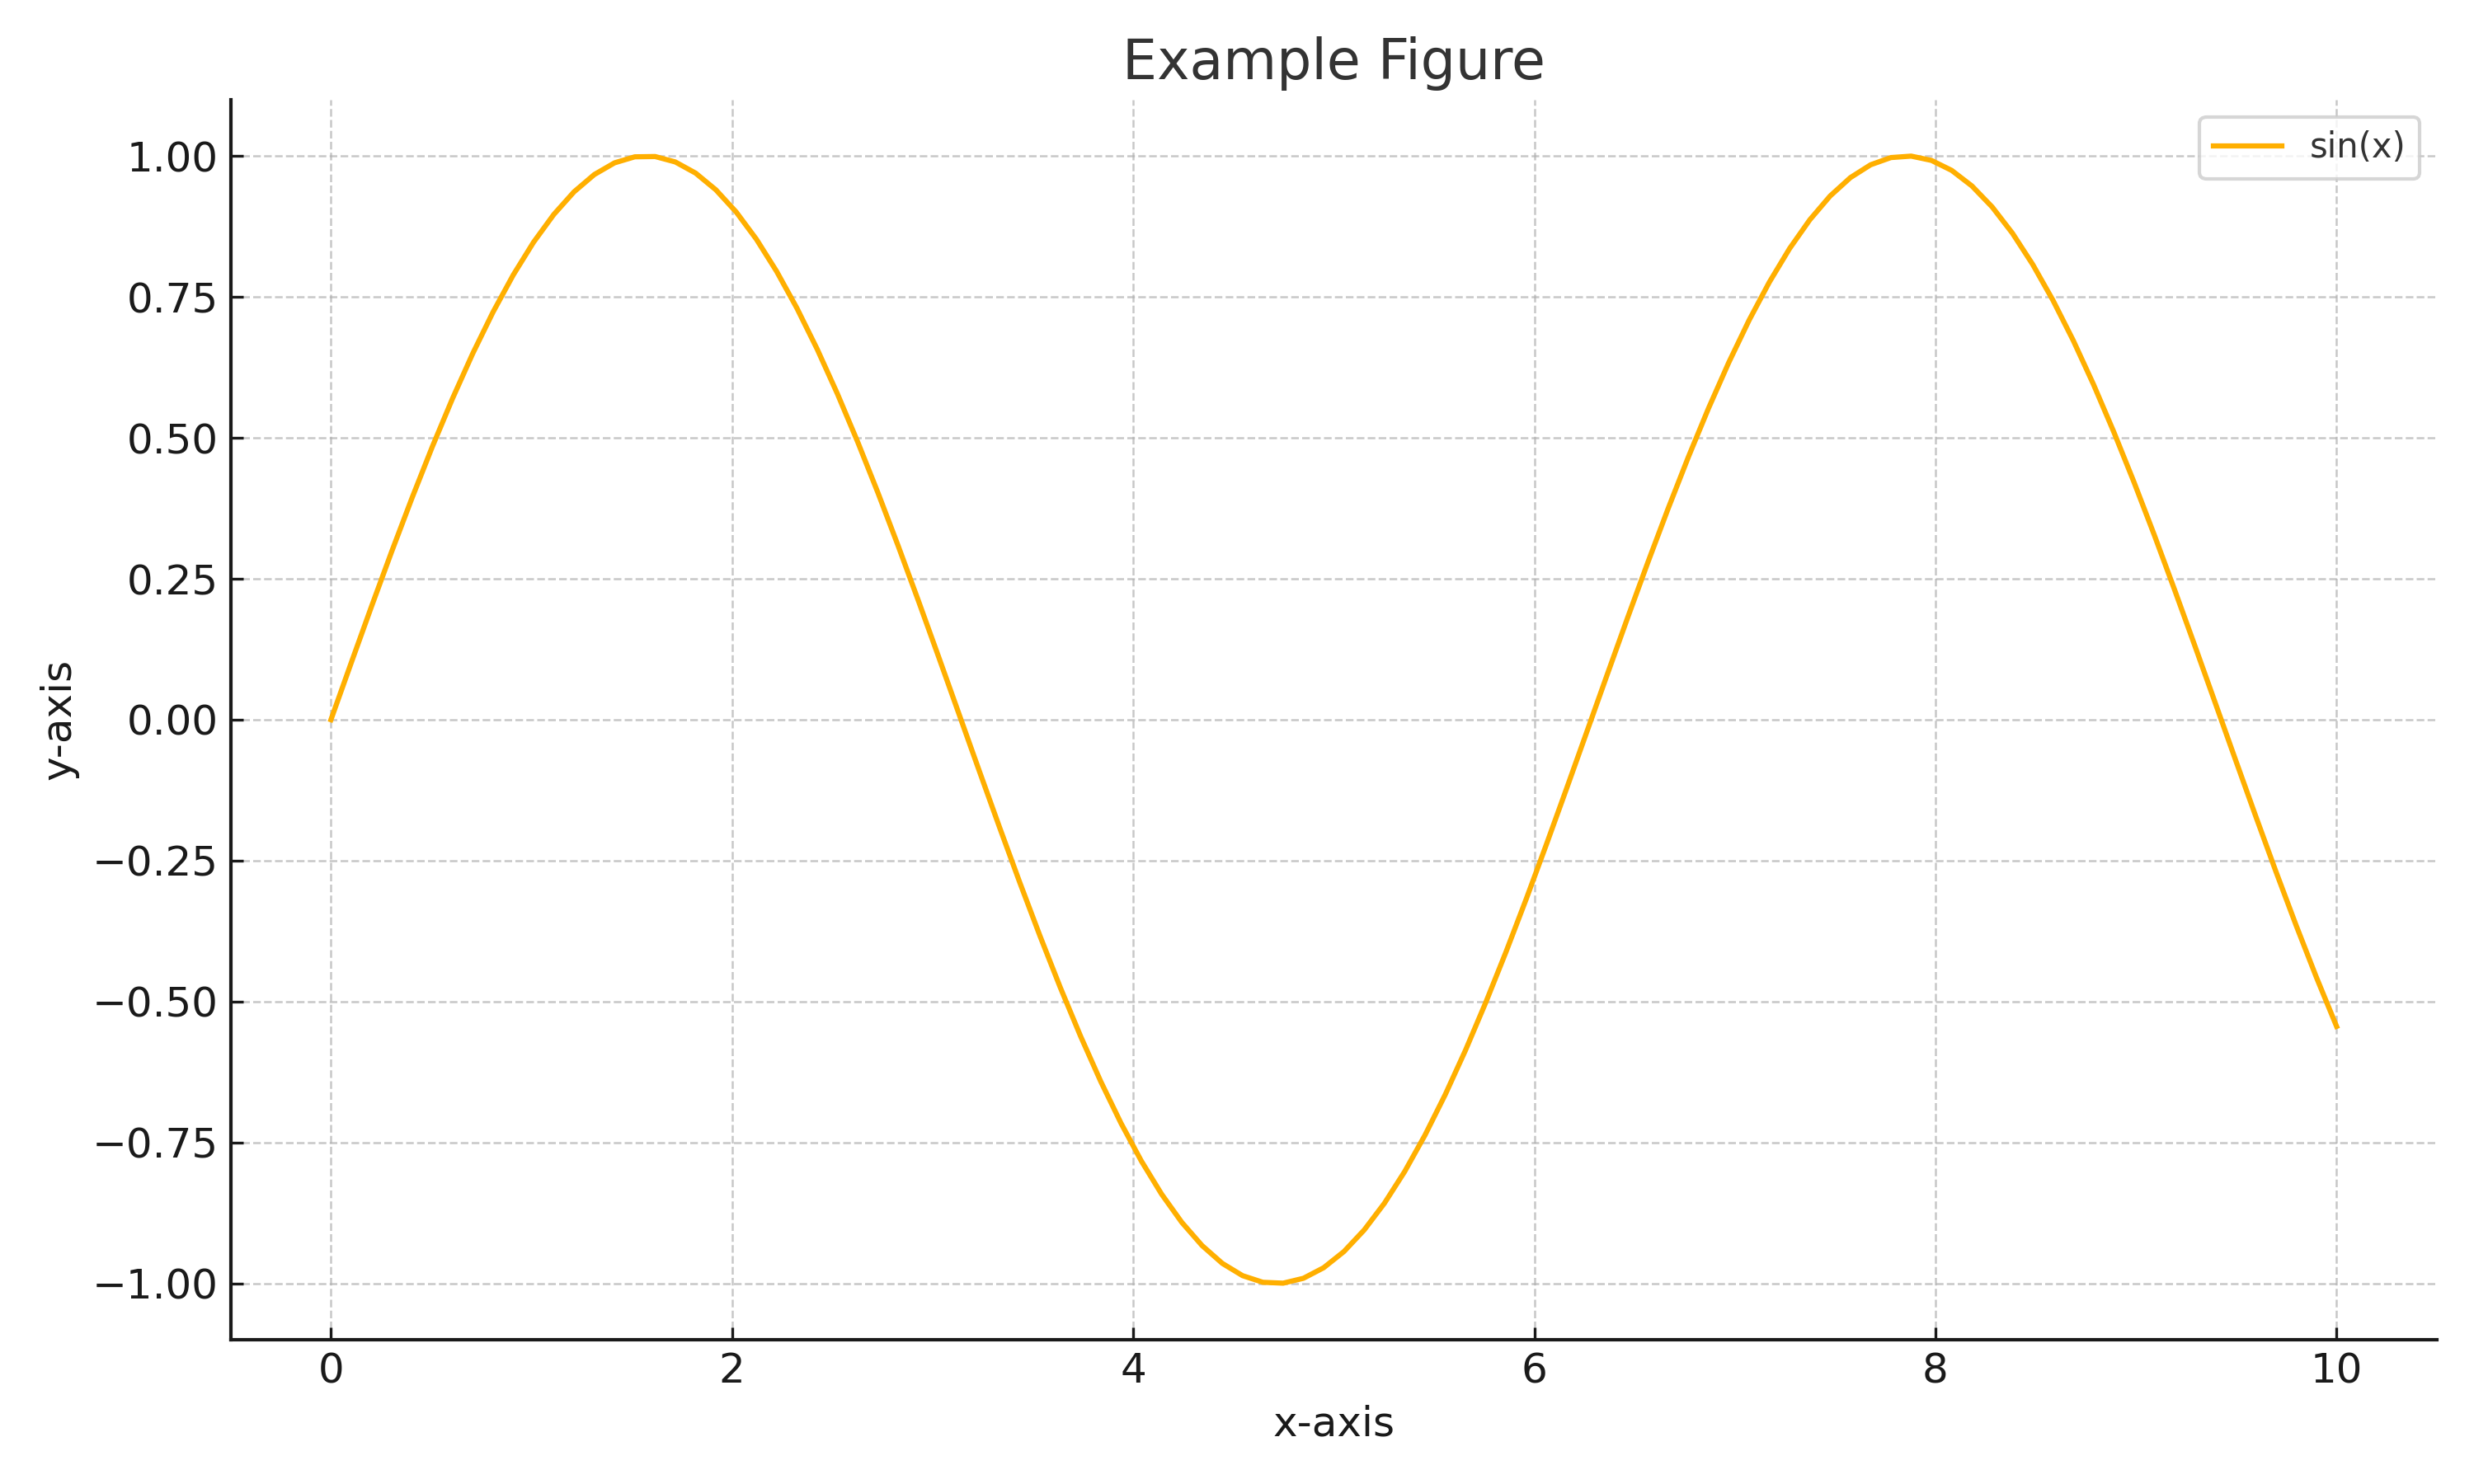
\includegraphics[width=0.8\textwidth]{example-figure.png}
    \caption{\textbf{Caption title.} Figure caption goes here.}
    \label{fig:example}
\end{figure}

% ----------------------------------------
% Example table
% Use \ref{tab:sample} to reference it in the text
\begin{table}[ht!]
    \centering
    \caption{\textbf{Sample table caption.} Table caption goes here.}
    \label{tab:sample}
    \begin{tabular}{|l|c|r|}
    \hline
    Header 1 & Header 2 & Header 3 \\
    \hline
    Value A & 123       & Text     \\
    Value B & 456       & More     \\
    \hline
    \end{tabular}
\end{table}

Here is a nice equation:
% ----------------------------------------
% Example equation
% Use \eqref{eq:einstein} to reference it in the text
\begin{equation}
    E = mc^2
    \label{eq:einstein}
\end{equation}

\bibliographystyle{unsrt}
\bibliography{references.bib}

\end{document}